\section{Catálogo de Productos (Servicios Turísticos)}

En Odoo, el término genérico es ``Producto'', pero para la agencia de viajes, estos serán nuestros \textbf{Servicios Turísticos} (tours, traslados, tickets, paquetes, etc.). Es fundamental configurar bien cada servicio para que las cotizaciones y el sitio web funcionen correctamente. 

En esta sección te mostramos paso a paso cómo dominar el ciclo de vida de un servicio (Crear, Leer, Actualizar, Borrar).

\subsection{1. Vista del Catálogo (Read)}

Para ver y buscar todos los servicios que ofrece la agencia, dirígete al módulo de Ventas y en el menú superior selecciona \textbf{Productos > Productos}. 

\begin{figure}[H]
    \centering
    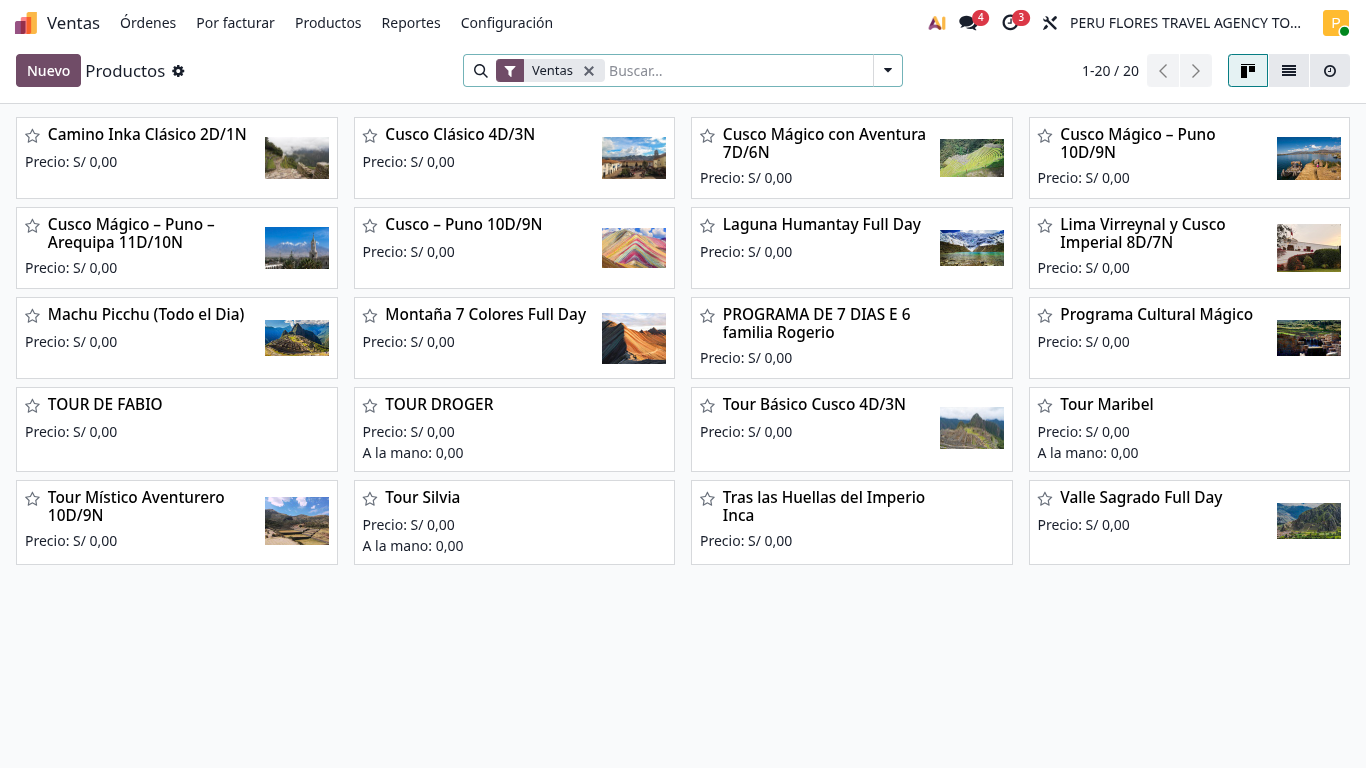
\includegraphics[width=0.9\textwidth]{assets/prod_det_01_lista.png}
    \caption{Vista Kanban (Read) del catálogo de servicios. Muestra foto, nombre y precio público.}
\end{figure}

Desde esta vista puedes usar la barra de búsqueda para encontrar un tour específico. Al hacer clic sobre cualquiera, ingresarás al detalle de ese servicio para leer toda su información.

\subsection{2. Crear un Nuevo Servicio (Create)}

Si la agencia lanza un nuevo tour o servicio al mercado, el primer paso es hacer clic en el botón \textbf{``Nuevo''} ubicado en la esquina superior izquierda.

\begin{figure}[H]
    \centering
    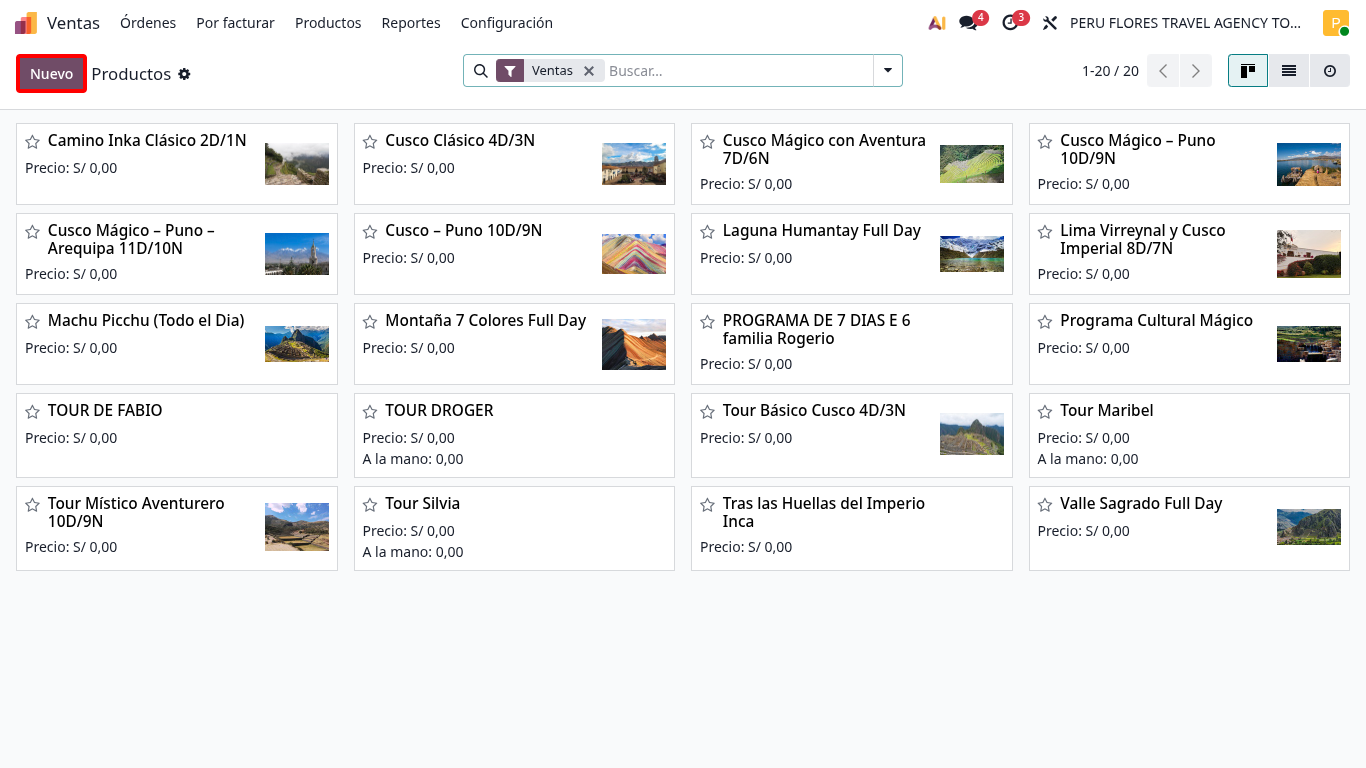
\includegraphics[width=0.9\textwidth]{assets/prod_det_02_boton_nuevo.png}
    \caption{El botón Nuevo (resaltado en rojo) inicia el flujo de creación (Create).}
\end{figure}

Al ingresar al formulario en blanco, el campo más vital que define el comportamiento del ítem en todo Odoo es el \textbf{Tipo de Producto}.

\begin{figure}[H]
    \centering
    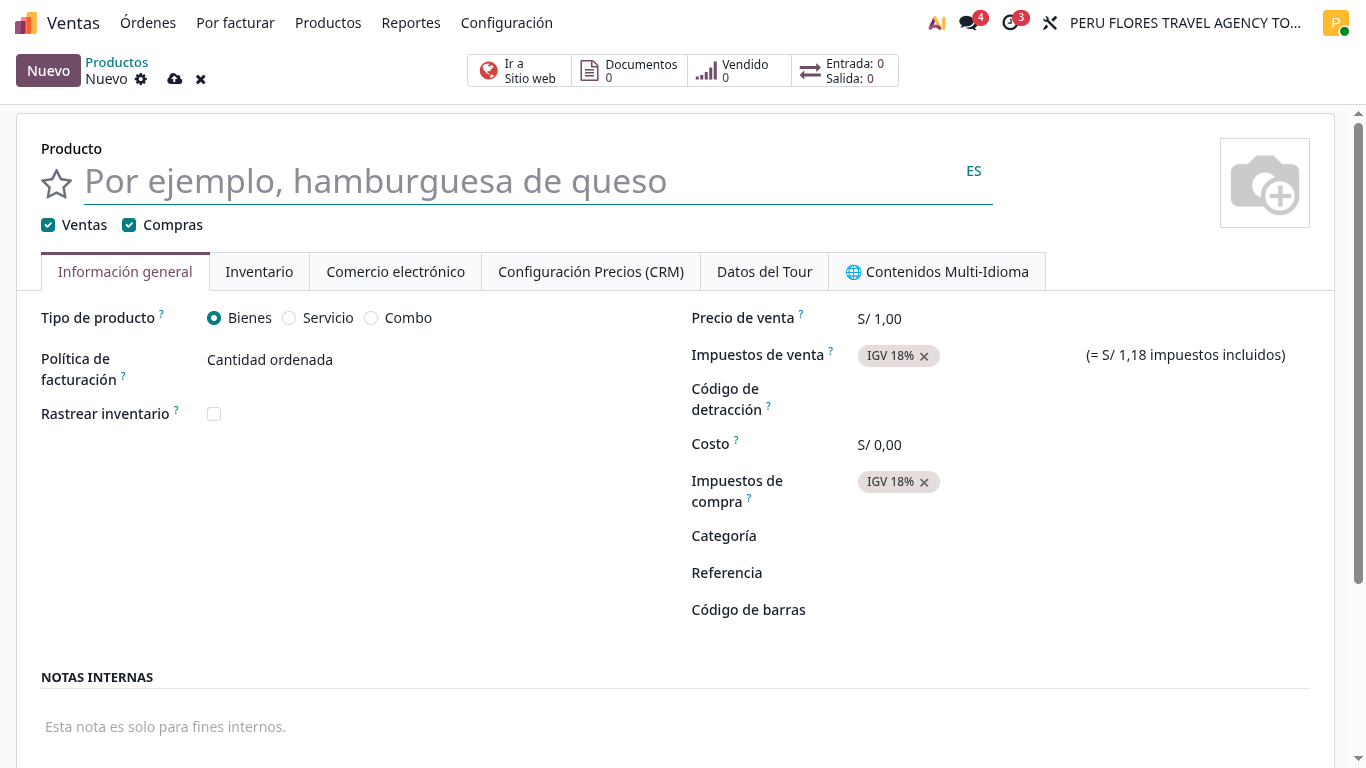
\includegraphics[width=0.9\textwidth]{assets/prod_det_03_form_crear.png}
    \caption{Formulario de creación. El campo Tipo de Producto está resaltado en rojo.}
\end{figure}

Debes llenar lo siguiente en la pestaña \textbf{Información General}:
\begin{itemize}
    \item \textbf{Nombre del Producto:} Escribe el nombre completo del tour (Ej: "Tour Montaña de 7 Colores - Full Day").
    \item \textbf{Puede ser vendido / Puede ser comprado:} Activa ambas casillas si lo vendes a clientes y también pagas a un operador externo por él.
    \item \textbf{Tipo de Producto:} \textbf{¡CRÍTICO!} Selecciona siempre \textbf{``Servicio''}. Nunca elijas "Almacenable", ya que la agencia no maneja stock físico de cajas o botellas.
\end{itemize}

\begin{figure}[H]
    \centering
    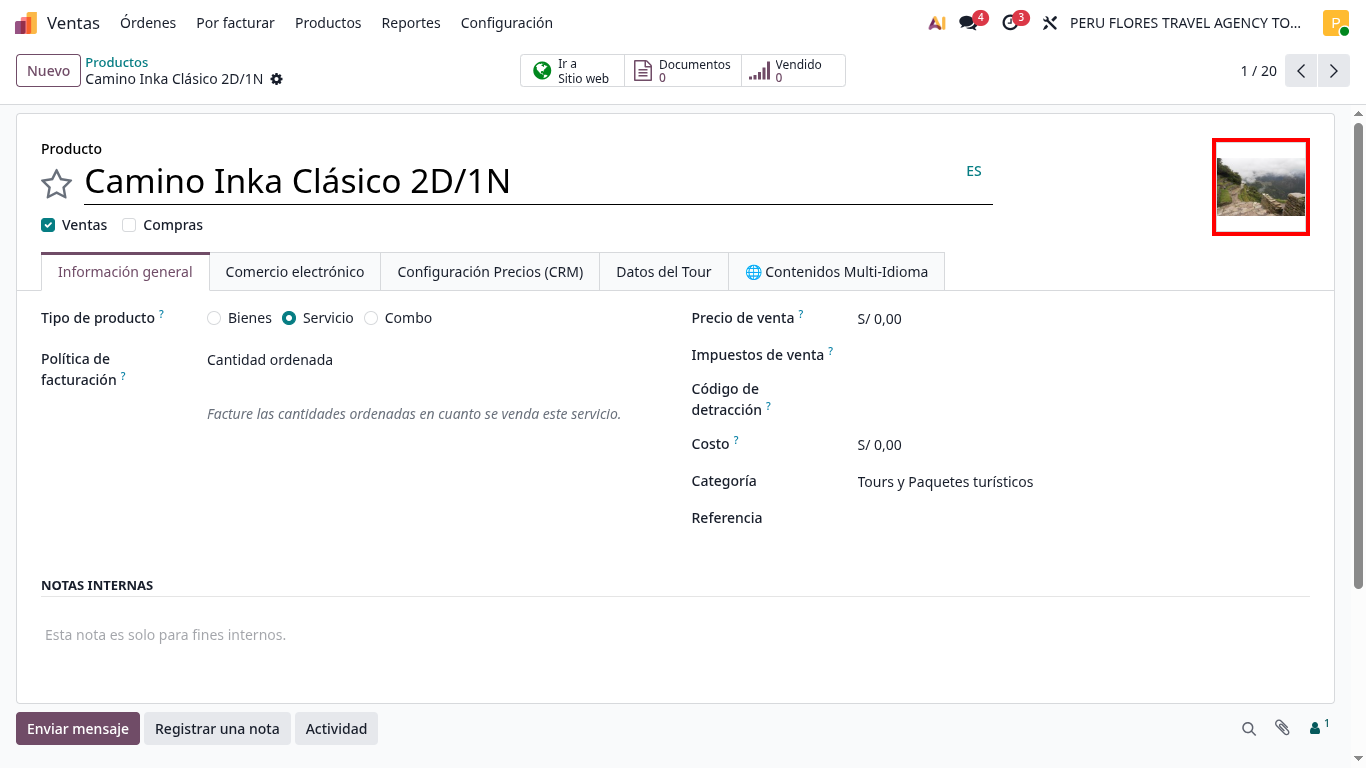
\includegraphics[width=0.9\textwidth]{assets/prod_det_07_foto.png}
    \caption{Agrega la Fotografía del Tour haciendo clic en la cámara (resaltada en rojo).}
\end{figure}

\textbf{Imagen Comercial:} Recuerda subir una foto representativa del tour. Esta foto aparecerá tanto en la cotización PDF como en la tienda web, dándole una apariencia profesional a la venta.

\subsection{3. Modificar Precios y Costos (Update)}

\begin{figure}[H]
    \centering
    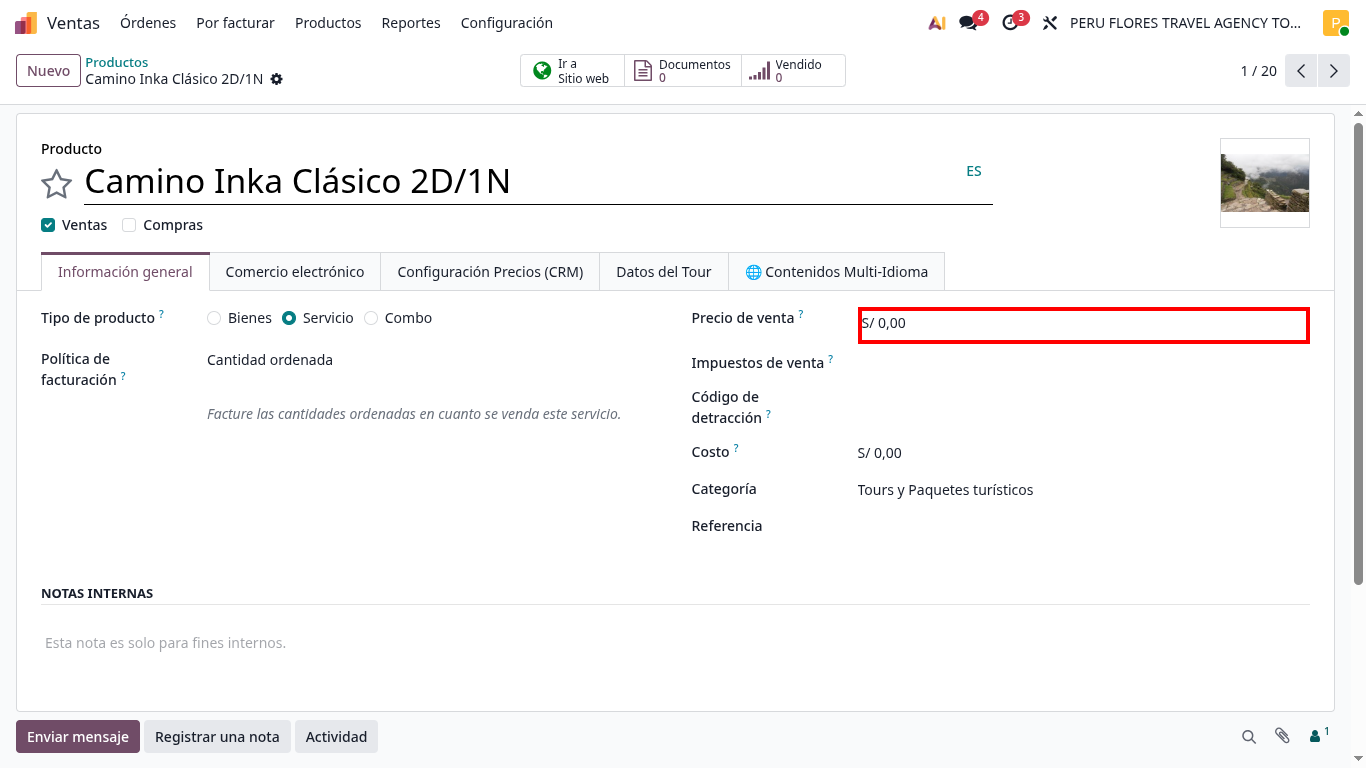
\includegraphics[width=0.9\textwidth]{assets/prod_det_04_precios.png}
    \caption{El campo Precio de Venta (resaltado en rojo). Este es el precio base que verán los pasajeros.}
\end{figure}

Si necesitas actualizar el \textbf{Precio de Venta} al público, simplemente borra el valor anterior y escribe la nueva tarifa. Esto actualizará automáticamente cualquier nueva cotización que los vendedores generen.

\begin{figure}[H]
    \centering
    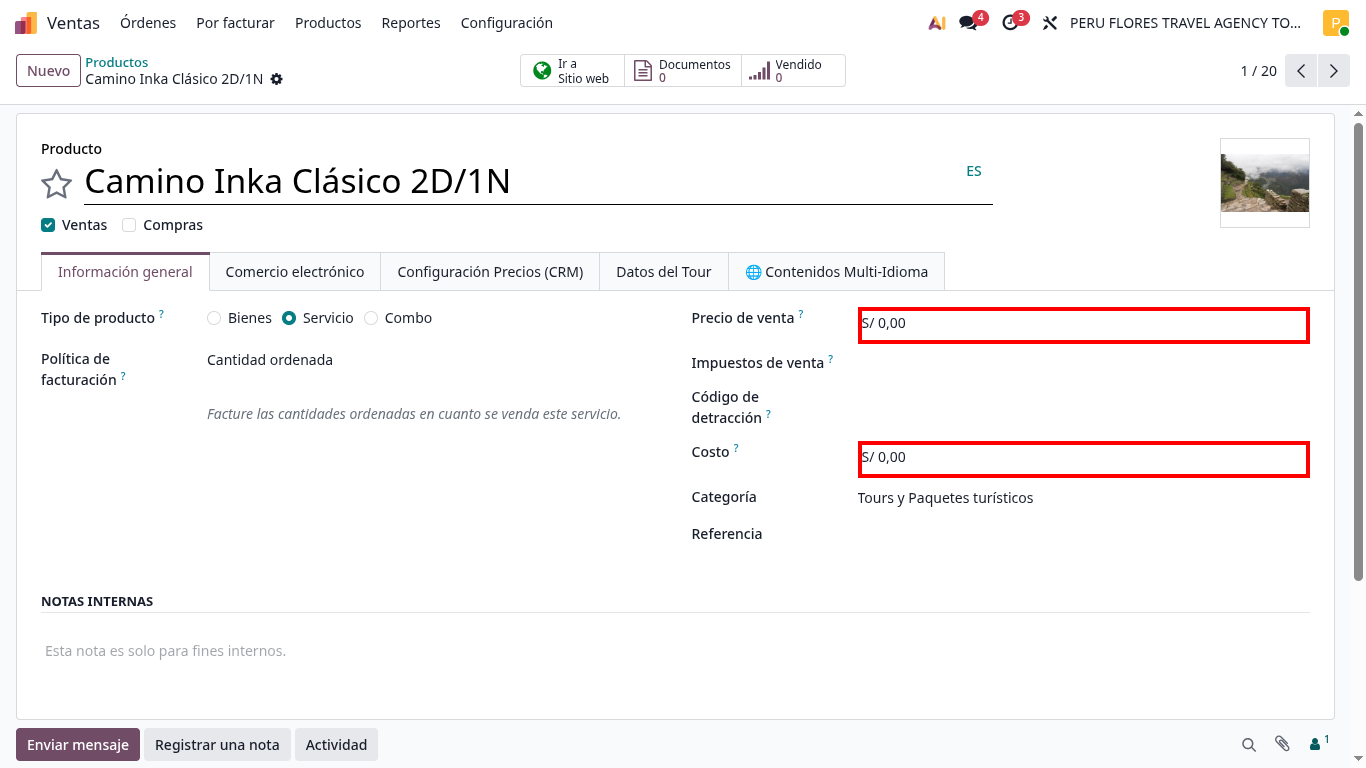
\includegraphics[width=0.9\textwidth]{assets/prod_det_05_costos.png}
    \caption{El campo Coste (resaltado en rojo). Este valor es confidencial.}
\end{figure}

Si el operador turístico nos sube la tarifa, actualiza el \textbf{Coste}. Odoo usa el Precio de Venta menos el Coste para calcular la rentabilidad real de la agencia.

\begin{figure}[H]
    \centering
    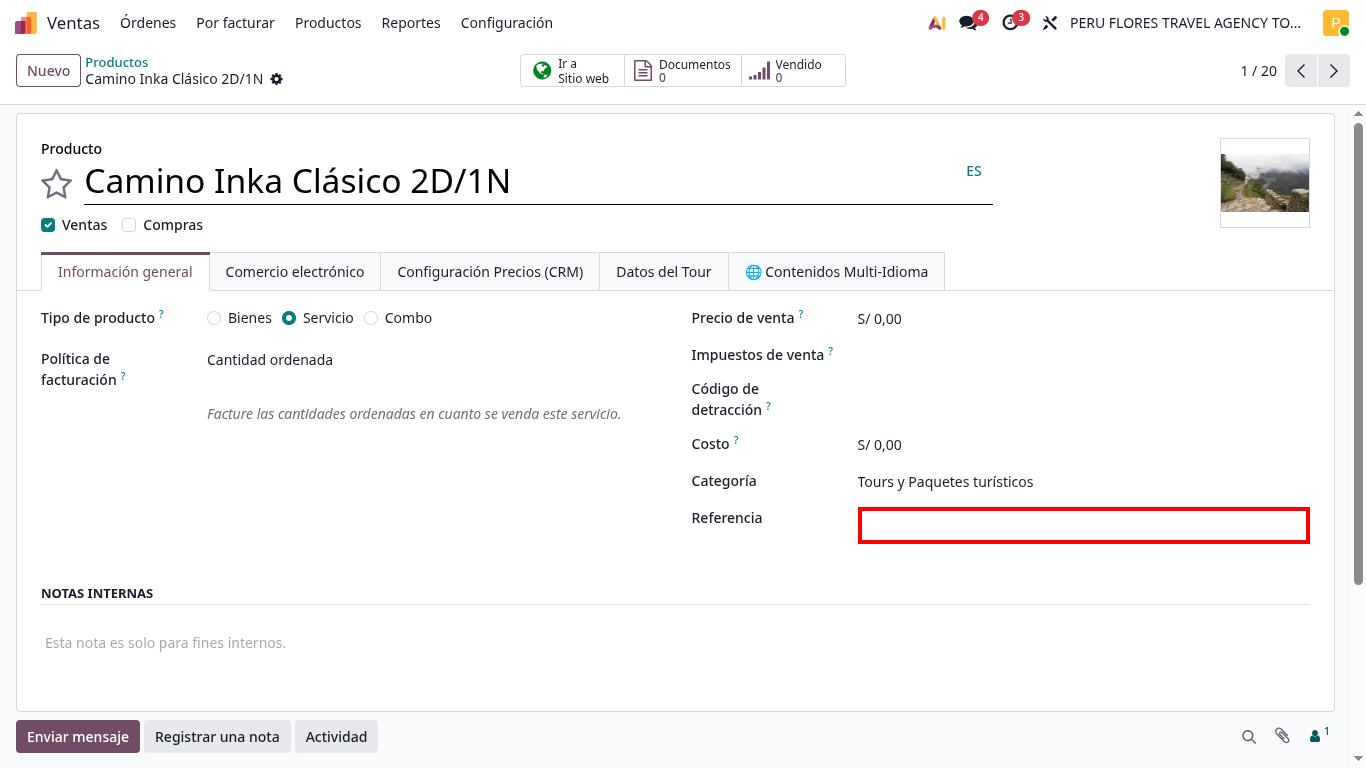
\includegraphics[width=0.9\textwidth]{assets/prod_det_10_sku.png}
    \caption{Referencia Interna (SKU), usado para códigos rápidos (Ej: TR-MAPI-01).}
\end{figure}

Adicionalmente, puedes usar la \textbf{Referencia Interna} para asignar códigos rápidos a los tours, facilitando la búsqueda a los vendedores.

\subsection{4. Configuración de Ventas y Web (Update Avanzado)}

Odoo tiene pestañas adicionales en la parte inferior del formulario para ajustar cómo se vende y cómo se muestra el servicio.

En la pestaña de Ventas encontrarás la \textbf{Descripción para ventas}. Lo que escribas aquí es exactamente lo que el cliente leerá debajo del nombre del tour cuando le envíes una proforma. Es ideal para resúmenes (Ej: "Incluye transporte privado, guía bilingüe y tickets de ingreso").

En la pestaña Comercio Electrónico defines la \textbf{Categoría del sitio web}. Si la agencia vende tours por internet, esto determina si el tour aparece en la página de "Cusco" o "Arequipa", por ejemplo.

\subsection{5. Pestañas Exclusivas de la Agencia (Datos Tour y Multi-Idioma)}

Para gestionar la gran cantidad de información que maneja un tour, hemos añadido pestañas exclusivas y personalizadas al sistema Odoo.

\subsubsection{Configuración Precios (CRM)}

\begin{figure}[H]
    \centering
    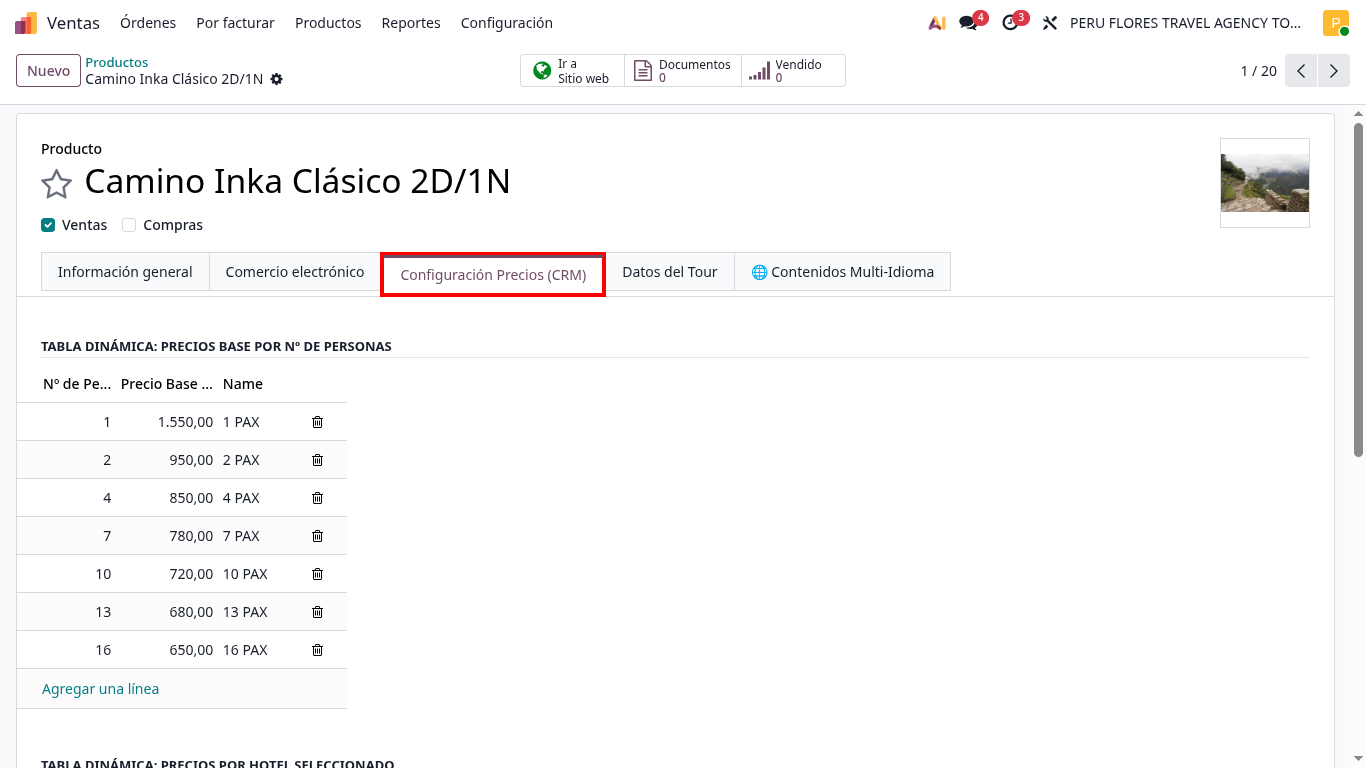
\includegraphics[width=0.9\textwidth]{assets/prod_det_11_precios_crm.png}
    \caption{Pestaña Configuración de Precios (CRM) con el contenido exacto.}
\end{figure}

Esta pestaña contiene opciones avanzadas de tarifario que se conectan directamente con el cotizador del CRM. Aquí podrás configurar precios especiales por grupos (por ejemplo, tarifa para 2 pasajeros, tarifa para grupos de 5+) o descuentos automáticos en fechas específicas.

\subsubsection{Datos del Tour}

\begin{figure}[H]
    \centering
    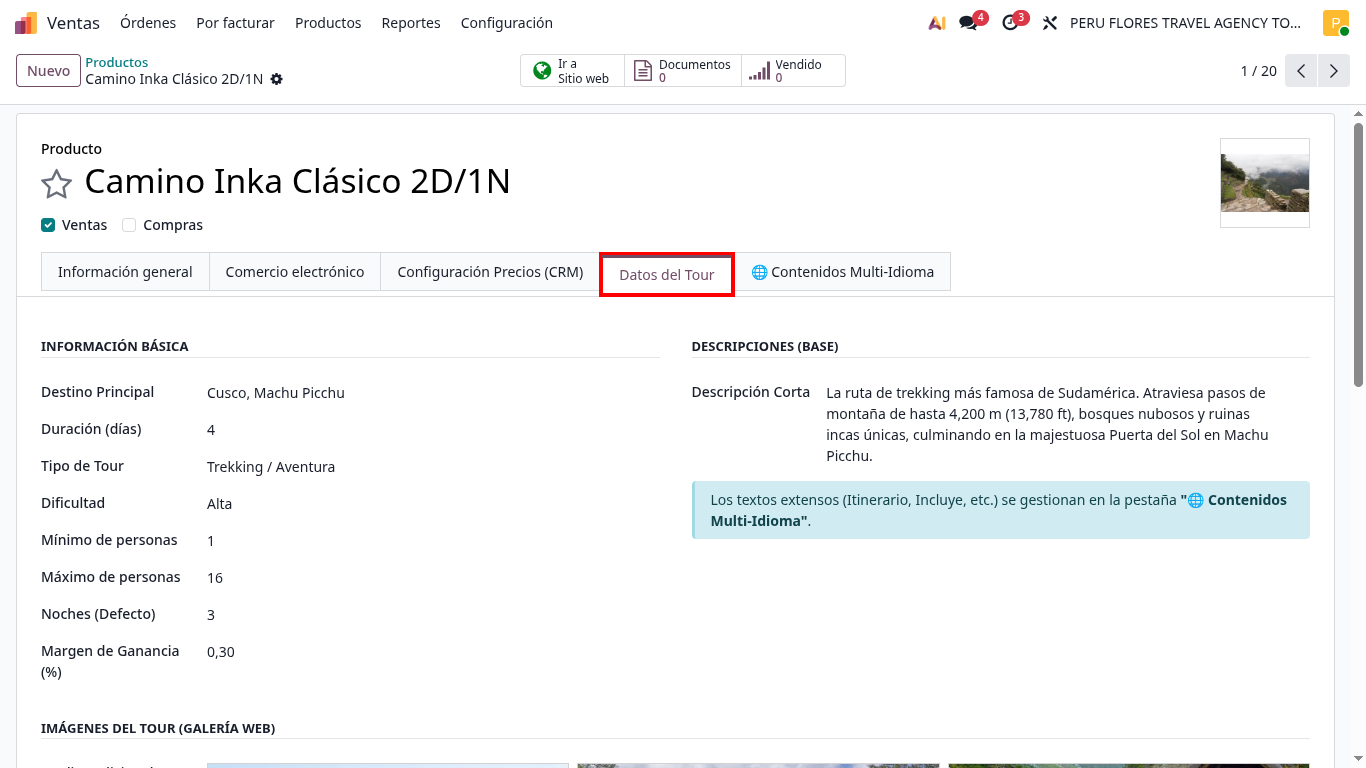
\includegraphics[width=0.9\textwidth]{assets/prod_det_12_datos_tour.png}
    \caption{Pestaña Datos del Tour con los campos técnicos requeridos.}
\end{figure}

Aquí debes llenar toda la ficha técnica del servicio. Por lo general, incluye campos críticos como el "Punto de Inicio", "Punto de Finalización", "Duración exacta en horas/días", "Dificultad del Trekking", e "Inclusiones/No Inclusiones". Toda esta información viaja automáticamente al PDF final que se le manda al cliente, por lo que su llenado es indispensable.

\subsubsection{Contenidos Multi-Idioma}

\begin{figure}[H]
    \centering
    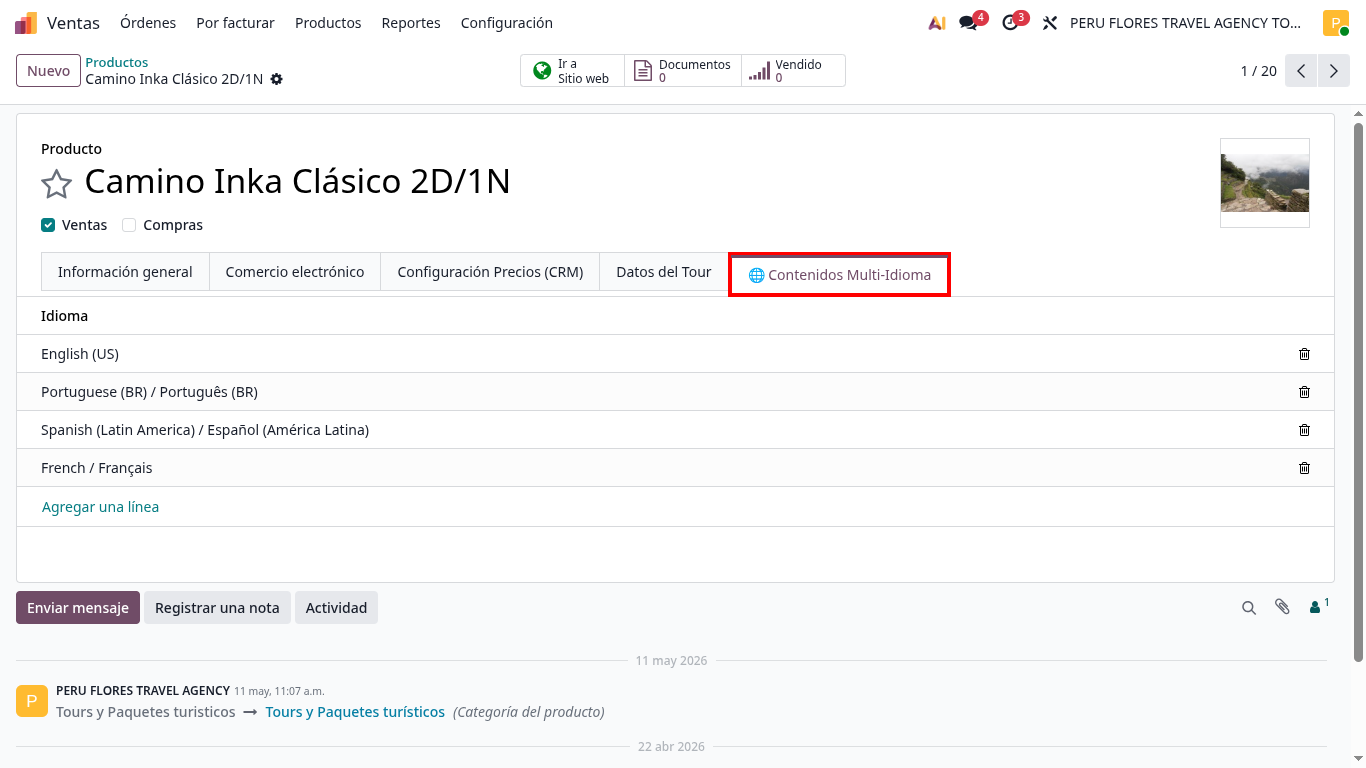
\includegraphics[width=0.9\textwidth]{assets/prod_det_13_multi_idioma.png}
    \caption{Pestaña Contenidos Multi-Idioma para el llenado de traducciones.}
\end{figure}

Si la agencia vende tours a pasajeros extranjeros, esta pestaña te salvará la vida. Aquí puedes agregar la traducción exacta del tour (al inglés, francés, portugués, etc.). Cuando envíes una proforma a un cliente que tiene el "Inglés" configurado en su perfil, Odoo tomará automáticamente la información de esta pestaña sin que tengas que traducir nada a mano.

\subsection{6. Archivar o Eliminar (Delete)}

Si un tour ya no se ofrece, debes removerlo del catálogo.

\begin{figure}[H]
    \centering
    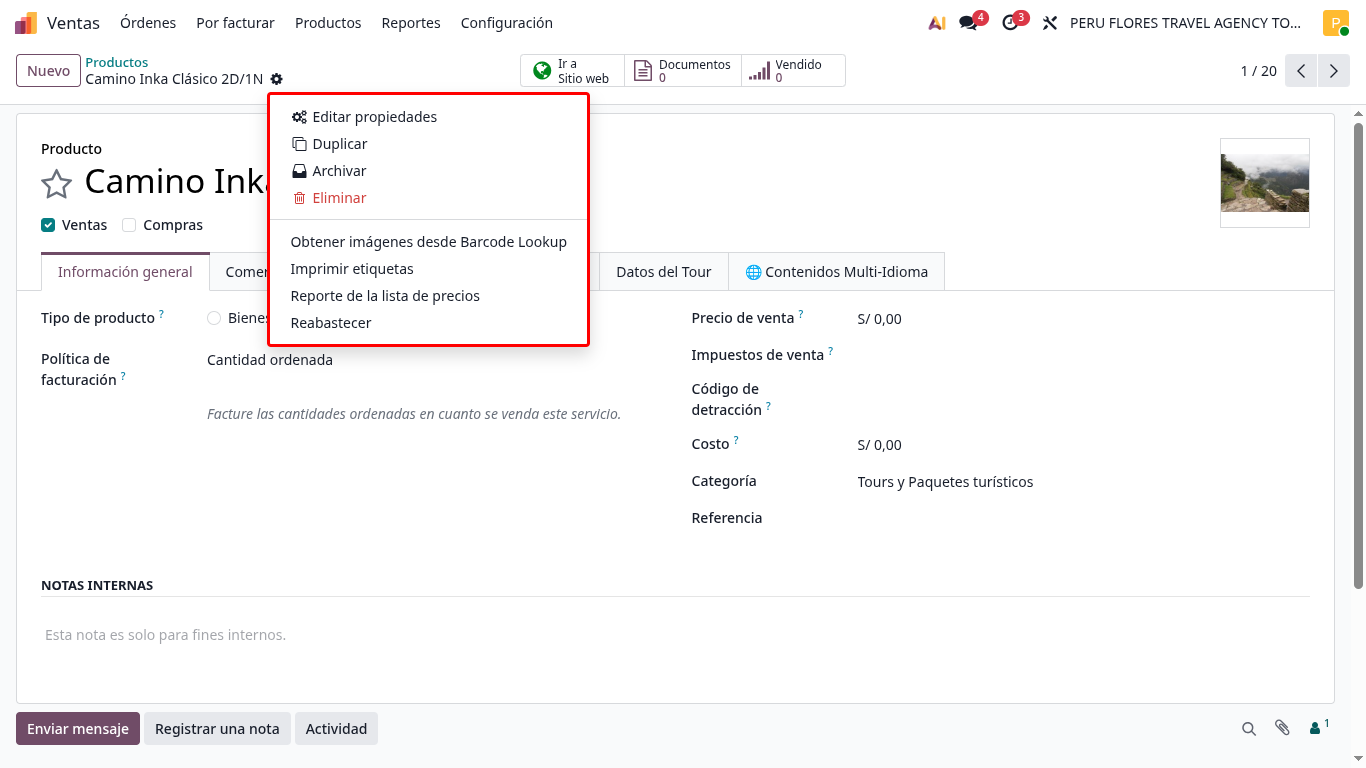
\includegraphics[width=0.9\textwidth]{assets/prod_det_06_archivar.png}
    \caption{Menú de Acción resaltando los botones de Archivar y Eliminar (Delete).}
\end{figure}

\begin{itemize}
    \item Para borrarlo, debes hacer clic en el ícono de engranaje (Acción) dentro del tour y elegir \textbf{``Eliminar''}.
    \item \textbf{¡Regla de Oro en Odoo!} El sistema no te dejará \textit{Eliminar} un servicio si ya ha sido cotizado o vendido a un pasajero (para proteger la contabilidad). 
    \item En ese caso, la práctica correcta es usar la opción \textbf{``Archivar''}. Al archivarlo, desaparece de la vista principal, pero se conserva en los registros históricos.
\end{itemize}
